% Task 3: find k. Values from PROBLEMS in Task3/ecdlp.py.
% CHECKED (python3, Task3/solution/ecdlp.py): the three k exist; they are the answer, so the figure does not show them
\documentclass[12pt,tikz,border=6pt]{standalone}
% Shared preamble of the task figures of Lecture 5 (based on Lecture02-ChaCha20/task-figures/common.tex).
% The roles take the colours of the elliptic-curves simulator (CryptographySimulators/elliptic-curves),
% so that the README figures and the simulator look the same:
%   secret (number or point): amber, public point: violet, Alice: blue, Bob: green,
%   Eve: red, ciphertext: brown, message: grey, a change or the unknown: orange.
\usepackage{lmodern}
\usepackage[T1]{fontenc}
\renewcommand{\familydefault}{\sfdefault}
\usepackage{amsmath,amssymb}
\usepackage{xcolor}
\usepackage{fontawesome5}
\usetikzlibrary{arrows.meta, calc, positioning, fit, decorations.pathreplacing, backgrounds}

% ---------- template and neutral ----------
\definecolor{DeepBlue}{HTML}{283593}
\definecolor{AccentOrange}{HTML}{EB5A14}
\definecolor{nInk}{HTML}{37474F}
\definecolor{nLine}{HTML}{90A4AE}
\definecolor{nLight}{HTML}{CFD8DC}
\definecolor{nFill}{HTML}{ECEFF1}
\definecolor{aExec}{HTML}{43A047}
\definecolor{aWrite}{HTML}{E53935}

% ---------- roles (the colours of the elliptic-curves simulator) ----------
\definecolor{rPriv}{HTML}{E2A60E}  \definecolor{rPrivBg}{HTML}{FDF3DC}  \definecolor{rPrivText}{HTML}{9A6B00}
\definecolor{rPub}{HTML}{8A5CD8}   \definecolor{rPubBg}{HTML}{F1EAFD}   \definecolor{rPubText}{HTML}{6A3FB8}
\definecolor{rAli}{HTML}{2F6FDB}   \definecolor{rAliBg}{HTML}{E5EDFB}
\definecolor{rBob}{HTML}{2FA84F}   \definecolor{rBobBg}{HTML}{E3F4E8}   \definecolor{rBobText}{HTML}{1E7E4F}
\definecolor{rEve}{HTML}{E5484D}   \definecolor{rEveBg}{HTML}{FDE9E9}
\definecolor{rCip}{HTML}{A8642A}   \definecolor{rCipBg}{HTML}{F7ECE0}
\definecolor{rMsg}{HTML}{BCC4CC}   \definecolor{rMsgBg}{HTML}{EEF1F4}
\definecolor{rChg}{HTML}{D9621C}   \definecolor{rChgBg}{HTML}{FCE8DA}

\tikzset{
  hw/.style={draw=nLine, thick, fill=nFill, text=nInk, rounded corners=3pt, align=center, inner sep=4pt},
  hwmain/.style={draw=nInk, thick, fill=nInk, text=white, rounded corners=3pt, align=center, inner sep=4pt},
  role/.style={draw=#1, thick, fill=#1Bg, text=nInk, rounded corners=3pt, align=center, inner sep=5pt},
  unk/.style={draw=rChg, thick, dashed, fill=white, text=rChg, rounded corners=3pt, align=center, inner sep=5pt,
    font=\bfseries},
  data/.style={-{Stealth}, very thick, nInk},
  note/.style={font=\small, text=nInk},
  person/.style={circle, fill=#1, draw=#1, text=white, minimum size=1.1cm, font=\Large, inner sep=0pt},
}
\newcommand{\personnode}[4]{%
  \node[person=#3] (#1) at (#2) {\faUser};
  \node[font=\small\bfseries, text=#3, below=0.06cm of #1] (#1lbl) {#4};}
\newcommand{\cogbox}[4]{%
  \node[hwmain, minimum width=#4, minimum height=1.1cm] (#1) at (#2) {};
  \node[text=white, font=\large, anchor=west] at ([xshift=0.2cm]#1.west) {\faCogs};
  \node[text=white, font=\small\bfseries] at ([xshift=0.3cm]#1.center) {#3};}

% ---------- the toy curve y^2 = x^3 + 2x + 2 mod 17 (as on the slides) ----------
% CHECKED: python3, all (x, y) with 0 <= x, y < 17 and y^2 = x^3 + 2x + 2 mod 17: these 18 points
\newcommand{\curvepts}{0/6,0/11,3/1,3/16,5/1,5/16,6/3,6/14,7/6,7/11,9/1,9/16,10/6,10/11,13/7,13/10,16/4,16/13}
% the grid of dots, in grid coordinates (1 unit = one step of x or y); draw it inside a scope
\newcommand{\gridbody}{%
  \foreach \x in {0,...,16} \foreach \y in {0,...,16} \fill[nLight] (\x,\y) circle (1.1pt);
  \draw[nLine, thick] (-0.7,-0.7) -- (16.7,-0.7);
  \draw[nLine, thick] (-0.7,-0.7) -- (-0.7,16.7);
  \foreach \v in {0,...,16} {
    \node[font=\tiny, text=gray, anchor=north] at (\v,-0.75) {\v};
    \node[font=\tiny, text=gray, anchor=east] at (-0.75,\v) {\v};
  }
  \node[font=\scriptsize, text=nInk, anchor=west] at (16.8,-0.7) {$x$};
  \node[font=\scriptsize, text=nInk, anchor=south] at (-0.7,16.8) {$y$};
  \foreach \x/\y in \curvepts \fill[nInk] (\x,\y) circle (3pt);}
% mark a point of the grid: \gmark[colour]{x,y}{label}{where the label goes}
\newcommand{\gmark}[4][rPub]{%
  \node[circle, draw=#1, line width=1.2pt, fill=#1, minimum size=9pt, inner sep=0pt] at (#2) {};
  \node[font=\scriptsize\bfseries, text=#1, #4, inner sep=1pt, outer sep=3pt, fill=white, fill opacity=0.85,
    text opacity=1, rounded corners=1pt] at (#2) {#3};}

\begin{document}
\pagecolor{white}
\begin{tikzpicture}[>=Stealth]
  % the idea: add G again and again until you hit T
  \node[font=\normalsize\bfseries, text=nInk, anchor=west] at (-0.6,2.0) {Start at $G$, keep adding $G$ until you reach $T$. Then $T = kG$: which $k$?};
  \foreach \lbl/\x/\i in {G/0/1, 2G/2.0/2, 3G/4.0/3, 4G/6.0/4} {
    \node[role=rPub, minimum width=1.2cm, font=\small\bfseries] (n\i) at (\x,0.9) {$\lbl$};
  }
  \foreach \a/\b in {1/2, 2/3, 3/4} \draw[data] (n\a) -- node[above, font=\scriptsize\bfseries, text=rChg] {$+G$} (n\b);
  \node[font=\large, text=nInk] (dots) at (7.6,0.9) {\ldots};
  \draw[data] (n4) -- (dots);
  \node[role=rPub, minimum width=1.2cm, font=\small\bfseries, draw=rChg, line width=1.6pt] (t) at (9.4,0.9) {$T$};
  \draw[data] (dots) -- node[above, font=\scriptsize\bfseries, text=rChg] {$+G$} (t);
  \node[unk, font=\small\bfseries] at (11.6,0.9) {$k = $ ?};

  % the three problems
  \node[font=\small\bfseries, text=nInk, anchor=west] at (-0.6,-0.35) {curve $y^2 = x^3 + ax + b \bmod p$};
  \node[font=\small\bfseries, text=rPubText] at (6.4,-0.35) {$G$};
  \node[font=\small\bfseries, text=rPubText] at (9.8,-0.35) {$T = kG$};
  \foreach \y/\bits/\p/\a/\b/\G/\T/\w in {-1.05/16/50459/13422/27875/{(1710, 42410)}/{(49665, 28300)}/0.5,
      -2.0/20/896107/808927/241789/{(119763, 855066)}/{(490971, 493613)}/1.0,
      -2.95/24/9788083/4564841/5425030/{(7065671, 8730247)}/{(619167, 4946861)}/1.5} {
    \node[hw, font=\scriptsize\ttfamily, anchor=west, text width=4.9cm, align=left] at (-0.6,\y)
      {\textbf{\bits\ bits}\ \ p = \p\\ a = \a, \ b = \b};
    \node[role=rPub, font=\scriptsize\ttfamily, minimum width=3.1cm] at (6.4,\y) {\G};
    \node[role=rPub, font=\scriptsize\ttfamily, minimum width=3.1cm] at (9.8,\y) {\T};
    \node[unk, font=\scriptsize\bfseries, inner sep=3pt] at (12.05,\y) {k = ?};
    \node[text=nInk, font=\normalsize] at (13.05,\y) {\faStopwatch};
    \node[unk, font=\scriptsize\bfseries, inner sep=3pt, anchor=west] at (13.35,\y) {? s};
  }
  \node[font=\scriptsize, text=gray, anchor=north west, align=left] at (-0.6,-3.55)
    {\texttt{add(P, Q, a, p)} is ready. Each $p$ is 4 bits longer: how many times longer does the search take?};
  \path (14.4,0) coordinate;
\end{tikzpicture}
\end{document}
